\documentclass[11pt]{article}

% ----------------------------------------------------------------------------
% ProPS-Twin -- Formal Technical & Research Report (Document 2)
% Supervisor-facing. Every quantitative claim verified against the repository.
% ----------------------------------------------------------------------------

\usepackage[utf8]{inputenc}
\usepackage[T1]{fontenc}
\usepackage{lmodern}
\usepackage[a4paper,margin=1in]{geometry}
\usepackage{microtype}
\usepackage{xcolor}
\usepackage{graphicx}
\usepackage{booktabs}
\usepackage{array}
\usepackage{longtable}
\usepackage{ragged2e}
\setlength{\emergencystretch}{3em}
\usepackage{amsmath}
\usepackage{amssymb}
\usepackage{enumitem}
\usepackage{tikz}
\usetikzlibrary{arrows.meta,positioning,shapes.geometric,fit,backgrounds,calc}
\usepackage{fancyhdr}
\usepackage{abstract}
\usepackage[hidelinks]{hyperref}
\usepackage{titlesec}
\usepackage{caption}

\definecolor{navy}{HTML}{1f2a44}
\definecolor{accent}{HTML}{2c4fb0}
\definecolor{green}{HTML}{3a7d2c}
\definecolor{cyan}{HTML}{127a6e}
\definecolor{red}{HTML}{b03030}
\definecolor{gray}{HTML}{555555}
\definecolor{panel}{HTML}{f2f2f2}
\definecolor{panelline}{HTML}{cccccc}

\hypersetup{colorlinks=true,linkcolor=accent,urlcolor=accent,citecolor=accent}

\newcommand{\code}[1]{\texttt{\small #1}}
\newcommand{\file}[1]{\textcolor{navy}{\texttt{\small #1}}}

\titleformat{\section}{\large\bfseries\color{navy}}{\thesection}{0.6em}{}
\titleformat{\subsection}{\normalsize\bfseries\color{accent}}{\thesubsection}{0.6em}{}

\pagestyle{fancy}
\fancyhf{}
\lhead{\small\textcolor{gray}{ProPS-Twin: Technical \& Research Report}}
\rhead{\small\textcolor{gray}{\thepage}}
\renewcommand{\headrulewidth}{0.3pt}

\captionsetup{font=small,labelfont=bf}

\begin{document}

% ---------------------------------------------------------------- title page
\begin{titlepage}
\centering
\vspace*{1.5cm}
{\color{navy}\rule{\linewidth}{1.4pt}}\\[10pt]
{\Huge\bfseries ProPS-Twin}\\[8pt]
{\LARGE An LLM-Guided Digital Twin for\\ IT/OT Security-Monitoring Evaluation}\\[10pt]
{\large Engineering and Research Report}\\[6pt]
{\color{navy}\rule{\linewidth}{1.4pt}}\\[1.4cm]

{\large\textbf{Implemented subsystem:}\\ simulated estate, scenario controller,
log-only evaluator, and live visualization}\\[1.2cm]

\begin{tabular}{rl}
\textbf{Document type} & Formal project report (supervisor-facing)\\[2pt]
\textbf{Repository} & \file{/CSE499} (modules \file{research/}, \file{services/}, \file{scripts/}, \file{viz/})\\[2pt]
\textbf{Language / runtime} & Python 3 (standard library only); vanilla JS front end\\[2pt]
\textbf{Verification} & 48 automated tests pass; results reproduced on 2026-11-19\\[2pt]
\textbf{Reward model} & $R=w_dD+w_cC+w_aA+w_rQ-w_fF-w_lL$\\
\end{tabular}

\vfill
{\small This report documents what has \emph{actually} been built and tested. It
distinguishes implemented, tested, observed, planned, and unimplemented
functionality throughout, and does not present intended behaviour as realised
behaviour.}\\[6pt]
{\small\color{gray}Compiled 2026-11-19.}
\end{titlepage}

% ---------------------------------------------------------------- abstract
\begin{abstract}
\noindent
ProPS-Twin is a digital twin of the security-monitoring estate of an
industrial-control (IT/OT) environment, built to serve as a reproducible
testbed for \emph{policy evaluation}: given a defensive policy, how well would
the monitored estate detect, contain, remain available under, and recover from a
security incident? The implemented subsystem models five estate components across
four security zones, drives them through seven scripted incident scenarios
(SC-01--SC-07) under a deterministic virtual clock, and emits a stream of
JSON-lines telemetry identical in form to what containerised services would log.
A \emph{log-only} evaluator then re-derives detections from that telemetry
alone---never consulting ground truth until after detection---and condenses each
run into a single scalar reward composed of six normalised dimensions: detection,
containment, availability, recovery, and false-positive and delay penalties. The
system is implemented entirely on the Python standard library, is byte
reproducible for a fixed seed, and is validated by 48 automated tests. A
standard-library HTTP/Server-Sent-Events backend and a dependency-free browser
interface provide a live view of a run and allow two policy levers---access
profile and alert threshold---to be varied and their effect on the reward
observed in real time. We report the measured reward for all seven scenarios,
demonstrate that the policy levers produce the intended, test-pinned changes in
the reward, and state precisely which parts of the broader design (Kubernetes
orchestration, a Wazuh SIEM, and the LLM-driven policy optimiser) remain scaffolded
rather than implemented.
\end{abstract}

\paragraph{Keywords.} digital twin; IT/OT security; intrusion detection
evaluation; reward design; reproducible simulation; prompted policy search;
Server-Sent Events.

\tableofcontents
\clearpage

% ================================================================ 1
\section{Introduction}
Security monitoring in industrial-control environments is hard to evaluate
empirically: one cannot inject malware into a running plant to measure a
detector, and captured incident data is scarce and sensitive. A \emph{digital
twin}---a software model faithful enough in its observable \emph{behaviour} to
stand in for the real system---offers a safe, repeatable alternative. ProPS-Twin
applies this idea not to the plant's physics but to its \emph{security telemetry}:
it models the log events the estate's components would emit, injects controlled
incidents, and scores how a defensive policy would have fared.

The project's name refers to \emph{prompted policy search} (ProPS): the intended
end state is an optimisation loop in which a large language model proposes
defensive policies and a scalar reward guides their refinement. This report
documents the foundation that loop requires and that has been built: the
simulated estate, the scenario engine, the reward, the evaluator, and a live
visualization. The optimiser itself is a later phase and is identified as such.

% ================================================================ 2
\section{Problem statement}
We require a means to answer, quantitatively and reproducibly: \emph{for a given
defensive policy $\pi$, how well does the monitored IT/OT estate perform against a
representative incident?} ``Well'' is multi-objective---detecting an incident,
containing it, keeping legitimate work available, recovering promptly, and not
drowning operators in false alarms are distinct and partly competing goals. The
problem is therefore (i) to generate realistic, labelled incident telemetry
without a live target; (ii) to score it with a detector that cannot see the
labels; and (iii) to combine the competing objectives into one comparable reward
that an optimiser can later climb.

% ================================================================ 3
\section{Objectives}
\begin{enumerate}[leftmargin=1.6em,nosep]
  \item Model a representative IT/OT estate as independently seedable component
        processes emitting a common event schema.
  \item Define a catalog of incident scenarios spanning both \emph{presence} and
        \emph{absence} detection, with explicit ground truth held outside the
        event stream.
  \item Implement a log-only evaluator that reproduces SIEM-style detection
        offline and computes a six-dimension reward.
  \item Guarantee determinism and reproducibility for a fixed seed.
  \item Expose the run through a dependency-free visualization with interactive
        policy levers.
  \item (Planned) wrap the same core in Kubernetes with a Wazuh SIEM and an
        LLM-driven policy optimiser.
\end{enumerate}

% ================================================================ 4
\section{System requirements}
\paragraph{Functional.} Deterministic multi-component telemetry generation;
scheduled incident injection on a virtual clock; a common validated event schema;
offline presence and absence detection with a tunable threshold; per-dimension and
aggregate reward computation; persistence of events and ground truth; a streaming
visualization with live policy levers.

\paragraph{Non-functional.} Runs on a bare workstation with no cluster and no
third-party Python packages (standard library only); byte-reproducible output; an
auditable ``honesty'' invariant (ground truth excluded from telemetry); sub-second
evaluation per scenario; a front end with no build step or CDN dependency.

% ================================================================ 5
\section{System architecture}
\label{sec:arch}
The architecture is a unidirectional pipeline (Figure~\ref{fig:arch}). A scenario
definition parameterises the Scenario Controller, which instantiates five
component models and advances a virtual clock over the evaluation window, flipping
component modes on schedule. Components emit events into a run-scoped Event Sink
that stamps and serialises them. The resulting event list is the \emph{sole}
input to the log-only evaluator, which produces a reward document. A
standard-library backend exposes the controller and evaluator over HTTP and
Server-Sent Events to a browser front end.

\begin{figure}[h]
\centering
\resizebox{\linewidth}{!}{%
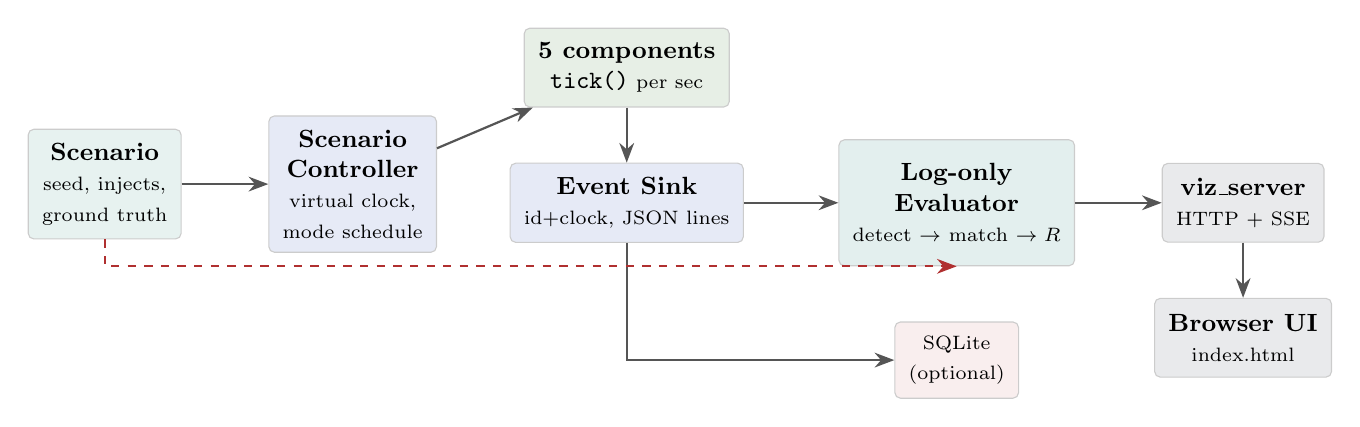
\begin{tikzpicture}[
  font=\small,
  box/.style={rectangle,rounded corners=2pt,draw=panelline,fill=panel,
              align=center,inner sep=5pt,minimum height=1.0cm},
  arr/.style={-{Stealth[length=2.5mm]},thick,draw=gray},
  ]
  \node[box,fill=cyan!10] (sc) {\textbf{Scenario}\\\scriptsize seed, injects,\\\scriptsize ground truth};
  \node[box,fill=accent!12,right=1.1cm of sc,minimum height=1.6cm] (ctrl)
      {\textbf{Scenario}\\\textbf{Controller}\\\scriptsize virtual clock,\\\scriptsize mode schedule};
  \node[box,fill=green!12,above right=0.1cm and 1.1cm of ctrl] (comp)
      {\textbf{5 components}\\\scriptsize \code{tick()} per sec};
  \node[box,fill=accent!12,below=0.7cm of comp] (sink) {\textbf{Event Sink}\\\scriptsize id+clock, JSON lines};
  \node[box,fill=cyan!12,right=1.2cm of sink,minimum height=1.6cm] (ev)
      {\textbf{Log-only}\\\textbf{Evaluator}\\\scriptsize detect $\to$ match $\to R$};
  \node[box,fill=navy!10,right=1.1cm of ev] (back) {\textbf{viz\_server}\\\scriptsize HTTP + SSE};
  \node[box,fill=navy!10,below=0.7cm of back] (ui) {\textbf{Browser UI}\\\scriptsize index.html};
  \node[box,fill=red!8,below=0.7cm of ev,minimum height=0.9cm] (db) {\scriptsize SQLite\\\scriptsize (optional)};

  \draw[arr] (sc)--(ctrl);
  \draw[arr] (ctrl)--(comp);
  \draw[arr] (comp)--(sink);
  \draw[arr] (sink)--(ev);
  \draw[arr] (ev)--(back);
  \draw[arr] (back)--(ui);
  \draw[arr] (sink.south)|-(db.west);
  \draw[arr,dashed,draw=red] (sc.south)|-(ev.south);
\end{tikzpicture}}
\caption{ProPS-Twin data-flow architecture. Telemetry (solid) and ground truth
(dashed) travel separately; they meet only inside the evaluator, after detections
have been computed.}
\label{fig:arch}
\end{figure}

% ================================================================ 6
\section{Methodology}
The methodology is \emph{behavioural simulation plus offline scoring}. Rather than
emulate packets or processes, each component is a small stochastic generator whose
output distribution shifts when the scenario places it in an attack mode. This
keeps the twin light and deterministic while preserving the only thing the
evaluator consumes: the log events. Detection is deliberately decoupled from
generation---it is a pure function of the event list---so that (a) the detector
cannot cheat, and (b) a policy can be re-scored against an existing run without
re-simulation. Competing objectives are reconciled by a weighted-sum reward whose
weights encode a stated priority ordering (detection $>$ containment $>$
availability $>$ recovery, with penalties for false alarms and delay).

% ================================================================ 7
\section{Implementation details}
\label{sec:impl}

\subsection{Event schema and the honesty invariant}
Every component emits one JSON object per line via a shared Event Sink
(\file{research/common/props\_log.py}). Each event carries a timestamp, a
component, an event type, a severity in
$\{\code{low},\code{medium},\code{high},\code{critical}\}$, a simulated state in
$\{\code{normal},\code{anomalous},\code{fault},\code{violation}\}$, a zone, the
policy version, and a free-form \code{details} payload. Crucially, no event
carries any label of whether it \emph{should} be detected; that information is the
ground-truth table, joined later by event ID. Event IDs are deterministic:
\code{event\_id = SHA256(experiment|component|seq)[:32]}, so a fixed seed yields a
byte-identical run.

\subsection{Component models}
The five components (\file{services/*/core.py}) share the pattern
\code{set\_mode()} / \code{tick(t, sink)} / \code{apply\_policy()} /
\code{state()}, and three expose a \code{probe()} for availability.
Table~\ref{tab:comp} summarises their behaviour and policy sensitivity.

\begin{table}[h]
\centering
\caption{Component models and their policy-sensitive behaviour.}
\label{tab:comp}
\small
\begin{tabular}{p{2.8cm} p{1.7cm} p{4.3cm} p{4.0cm}}
\toprule
\textbf{Component} & \textbf{Zone} & \textbf{Emits} & \textbf{Policy lever}\\
\midrule
idmz-gateway & idmz
  & protocol anomaly, jump-host crossing, unauthenticated access, heartbeats
  & access profile sets \code{contained}; lockdown fails probes\\
boundary-firewall & idmz
  & packet-storm volume, drop-rate, MAC spoofing, heartbeats
  & rate limit $\le 60$ sets \code{contained}\\
plc-edge & field
  & watchdog heartbeat, firmware integrity, I/O violations
  & none (v1)\\
eng-station & supervisory
  & compliance status, periodic audit log, privileged command
  & access profile sets \code{contained}\\
telemetry-forwarder & control
  & forwarding health, memory/jitter; answers probes
  & recovery timeout bounds $Q$; buffer drain delays recovery\\
\bottomrule
\end{tabular}
\end{table}

\subsection{Scenario Controller}
\file{research/scenario\_controller/controller.py} validates the scenario, builds
the components from the global seed, and steps a virtual clock
(\code{EPOCH = 2026-01-01}) one tick per simulated second over the evaluation
window. It expands each scheduled action into a set-at/restore-at pair, applies
modes at the right tick, and, for scenarios that define probes, polls availability
targets at the configured interval. It returns the experiment ID, the collected
events, and the ground-truth rows, and can optionally persist both to SQLite.

\subsection{Log-only evaluator}
\file{research/evaluation/engine.py} implements two detection paths.
\emph{Presence} detection (\code{detect\_presence}) fires on a drop-rate signal
that crosses a cutoff derived from the \code{alert\_threshold} policy, or on any
event whose simulated state is anomalous/fault/violation; probe and
absence-monitored event types are excluded. \emph{Absence} detection
(\code{detect\_coverage\_gap}) finds the longest stretch in which a required
periodic signal is missing and raises a coverage alert if it exceeds the timeout.
Alerts are matched to ground truth by event ID and window to yield true
positives, false positives, and misses; containment is read from the
\code{contained} flags on labelled events; availability from probe results; and
recovery from the settle time after a fault window. Weighted components are
combined by \file{metrics.py}.

% ================================================================ 8
\section{Technology stack}
\begin{longtable}{>{\RaggedRight\arraybackslash}p{3.4cm} >{\RaggedRight\arraybackslash}p{3.0cm} >{\RaggedRight\arraybackslash}p{7.4cm}}
\toprule
\textbf{Technology} & \textbf{Where} & \textbf{Role}\\
\midrule\endhead
Python 3 standard library & simulation, evaluation, backend
  & \code{random} (seeded generators), \code{hashlib} (deterministic IDs),
    \code{datetime} (virtual clock), \code{json}, \code{sqlite3} (optional
    persistence), \code{http.server} / \code{ThreadingHTTPServer} (backend),
    \code{urllib} (query parsing). No third-party package is required to run or
    test the core.\\
PyYAML & scenario loading (optional)
  & \code{catalog.load()} reads canonical YAML when PyYAML is present and falls
    back to an in-code mirror otherwise, so the core runs without it.\\
Server-Sent Events (SSE) & \file{viz\_server.py} $\to$ browser
  & one-way event streaming: a \code{meta} event, one \code{tick} per simulated
    second, then \code{reward} and \code{done}.\\
Vanilla JavaScript + EventSource & \file{viz/index.html}
  & front end with no framework, build step, or CDN; consumes the SSE stream or
    replays a baked dataset offline.\\
CSS (Moonfly palette) & \file{viz/index.html}
  & terminal-themed styling.\\
pytest & \file{tests/}
  & test runner (development dependency only).\\
Kubernetes (kind) + Calico; Wazuh; reportlab & \emph{planned / tooling}
  & orchestration, SIEM, and PDF generation; \emph{not} part of the executed
    simulation path (Section~\ref{sec:status}).\\
\bottomrule
\end{longtable}

% ================================================================ 9
\section{Simulation design}
Each component owns one or more independent RNG streams seeded as
\code{Random(seed + offset)}, so components are mutually independent yet
collectively reproducible, and a component's probe stream never perturbs its
telemetry stream. Normal operation emits heartbeats drawn from a clamped Gaussian;
periodic \emph{near-miss} events raise a benign signal slightly---below the
default cutoff---so that an over-sensitive policy generates false positives on
them. Incident modes replace the heartbeat with incident telemetry. The
forwarder additionally models non-instantaneous recovery: on leaving a degraded
mode it owes a bounded buffer-drain before it reports healthy, which is what the
recovery dimension measures.

\begin{figure}[h]
\centering
\resizebox{\linewidth}{!}{%
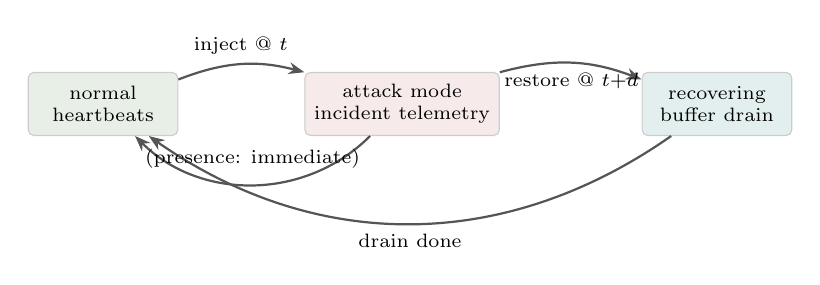
\begin{tikzpicture}[
  font=\scriptsize,node distance=0.9cm,
  st/.style={rectangle,rounded corners=2pt,draw=panelline,fill=panel,
             minimum width=1.9cm,minimum height=0.8cm,align=center},
  arr/.style={-{Stealth[length=2mm]},thick,draw=gray},
  ]
  \node[st,fill=green!12] (n) {normal\\\scriptsize heartbeats};
  \node[st,fill=red!10,right=1.6cm of n] (a) {attack mode\\\scriptsize incident telemetry};
  \node[st,fill=cyan!12,right=1.8cm of a] (r) {recovering\\\scriptsize buffer drain};
  \draw[arr] (n) to[bend left=18] node[above]{inject @ $t$} (a);
  \draw[arr] (a) to[bend left=18] node[below]{restore @ $t{+}d$} (r);
  \draw[arr] (r) to[bend left=35] node[below]{drain done} (n);
  \draw[arr] (a) to[bend left=45] node[above,yshift=2pt]{(presence: immediate)} (n);
\end{tikzpicture}}
\caption{Component mode lifecycle. Presence scenarios return directly to normal at
the end of the window; the forwarder (SC-07) passes through a bounded recovery
state first.}
\label{fig:lifecycle}
\end{figure}

% ================================================================ 10
\section{Data generation and processing pipeline}
The pipeline (Figure~\ref{fig:arch}) is: \emph{inject} a mode at tick $t$;
\emph{emit} events for every component each tick; \emph{stamp} and
\emph{serialise} each event with a deterministic ID; \emph{collect} the events;
\emph{detect} from telemetry alone; \emph{match} detections to ground truth;
\emph{reduce} to the six dimensions and the reward; and \emph{stream} the ticks
and reward to the UI. Because detection is pure over the event list, the same
captured run can be re-scored under a different policy (e.g.\ a different alert
threshold) without re-simulating---a property the interactive levers rely on.

% ================================================================ 11
\section{The seven scenarios}
The catalog (\file{configs/scenarios/}, mirrored in \file{catalog.py}) is given in
Table~\ref{tab:scen}. Each scenario fixes a seed, an injected incident with a time
window, the ground truth (presence or absence), and the evaluation window
($[0,120]$ seconds throughout).

\begin{table}[h]
\centering
\caption{Scenario catalog. Type is the detection style; the final column names the
dimension the scenario is designed to exercise.}
\label{tab:scen}
\footnotesize
\begin{tabular}{p{0.9cm} p{4.1cm} p{2.3cm} p{1.1cm} p{1.0cm} p{2.4cm}}
\toprule
\textbf{ID} & \textbf{Incident} & \textbf{Component} & \textbf{Window} & \textbf{Type} & \textbf{Exercises}\\
\midrule
SC-01 & Non-whitelisted inter-zone protocol & idmz-gateway & $[30,50]$ & presence & detection\\
SC-02 & Broadcast/multicast packet storm & boundary-firewall & $[40,55]$ & presence & detection, containment\\
SC-03 & Privilege escalation & eng-station & $[50,51]$ & presence & containment (uncontained)\\
SC-04 & Zone-segmentation violation & idmz-gateway & $[35,45]$ & presence & containment (lever)\\
SC-05 & Missing security-audit log & eng-station & $[40,70]$ & absence & coverage, delay\\
SC-06 & Unauthenticated remote access & idmz-gateway & $[45,53]$ & presence & containment\\
SC-07 & Heartbeat pause then recovery & telemetry-forwarder & $[40,60]$ & absence & availability, recovery\\
\bottomrule
\end{tabular}
\end{table}

% ================================================================ 12
\section{Evaluation methodology and metrics}
\label{sec:metrics}
All component metrics are pure functions of counts or lists
(\file{research/evaluation/metrics.py}) and normalised to $[0,1]$. Let $TP$, $FP$,
$FN$ be true/false positives and misses, $G=TP+FN$ the ground-truth positives, and
$B$ the benign-event count.

\begin{align}
D &= \frac{TP}{G} \quad (G{=}0 \Rightarrow 1), &
C &= \frac{\text{contained}}{\text{total}} \quad (\text{total}{=}0 \Rightarrow 1),\\
A &= \frac{\text{probe\_ok}}{\text{probes}} \quad (\text{probes}{=}0 \Rightarrow 1), &
Q &= 1-\min\!\Big(1,\tfrac{t_\text{rec}}{T_\text{budget}}\Big) \quad (\text{no fault}\Rightarrow 1),\\
F &= \frac{FP}{B} \quad (B{=}0 \Rightarrow 0), &
L &= \min\!\Big(1,\tfrac{1}{W}\cdot\tfrac{\sum_i \min(d_i,W) + FN\cdot W}{|d|+FN}\Big).
\end{align}

The reward aggregates them with the handbook weights
(\file{configs/evaluation/reward.yaml}, identical to \code{DEFAULT\_WEIGHTS}):
\begin{equation}
R(\pi) = \underbrace{0.30}_{w_d}D + \underbrace{0.25}_{w_c}C + \underbrace{0.20}_{w_a}A + \underbrace{0.10}_{w_r}Q - \underbrace{0.10}_{w_f}F - \underbrace{0.05}_{w_l}L .
\label{eq:R}
\end{equation}
The positive weights sum to $0.85$, so $R\in(-0.15, 0.85]$ and the maximum
attainable reward is $\mathbf{0.85}$.

\paragraph{Detection threshold.} The \code{alert\_threshold}
$\tau\in[1,5]$ maps to a drop-rate cutoff $c(\tau)=0.05+\tfrac{\tau-1}{4}(0.25-0.05)$;
the baseline $\tau=3$ gives $c=0.15$. Incident bumps (e.g.\ $+0.20$ at the
gateway, $+0.35$ for a storm) exceed it; near-miss bumps ($\le 0.12$) do not,
until $\tau$ is lowered.

\paragraph{A verified modelling choice.} For presence incidents the matched
detection delay is set to zero in the current implementation
(\file{engine.py}: \code{matched\_delays.extend(0.0 for \_ in matched)}). Only
absence detections contribute a non-zero delay, equal to the coverage timeout.
Consequently $L>0$ arises only in SC-05 and SC-07. This is a deliberate property
of the log-only (fast-mode) evaluator and is documented here so that detection
\emph{latency} is not over-interpreted.

% ================================================================ 13
\section{Experimental results}
\label{sec:results}
Table~\ref{tab:results} reports the reward and its components for all seven
scenarios under the baseline policy, reproduced on 2026-11-19 via
\code{python3 scripts/evaluate\_local.py all}.

\begin{table}[h]
\centering
\caption{Baseline results (access profile \code{standard}, $\tau=3$). Values are
exact program output.}
\label{tab:results}
\small
\begin{tabular}{l r rrrrrr rrr}
\toprule
\textbf{Scenario} & \textbf{R} & \textbf{D} & \textbf{C} & \textbf{A} & \textbf{Q} & \textbf{F} & \textbf{L} & \textbf{TP} & \textbf{G} & \textbf{FP}\\
\midrule
SC-01 & 0.8500 & 1.000 & 1.000 & 1.000 & 1.000 & 0.000 & 0.000 & 20 & 20 & 0\\
SC-02 & 0.8500 & 1.000 & 1.000 & 1.000 & 1.000 & 0.000 & 0.000 & 15 & 15 & 0\\
SC-03 & 0.6000 & 1.000 & 0.000 & 1.000 & 1.000 & 0.000 & 0.000 & 1 & 1 & 0\\
SC-04 & 0.6000 & 1.000 & 0.000 & 1.000 & 1.000 & 0.000 & 0.000 & 10 & 10 & 0\\
SC-05 & 0.8479 & 1.000 & 1.000 & 1.000 & 1.000 & 0.000 & 0.042 & 1 & 1 & 0\\
SC-06 & 0.6000 & 1.000 & 0.000 & 1.000 & 1.000 & 0.000 & 0.000 & 8 & 8 & 0\\
SC-07 & 0.7879 & 1.000 & 1.000 & 0.750 & 0.900 & 0.000 & 0.042 & 1 & 1 & 0\\
\bottomrule
\end{tabular}
\end{table}

\subsection{Policy-lever experiments}
The following effects are both reproduced and pinned by automated tests
(\file{tests/unit/test\_evaluation.py}):
\begin{itemize}[leftmargin=1.6em,nosep]
  \item \textbf{Containment lever (SC-04).} Access profile \code{standard} yields
        $C=0.0$, $R=0.60$; \code{strict} yields $C=1.0$, $R=0.85$. A single policy
        change recovers the full containment weight.
  \item \textbf{Detection/false-positive trade-off (SC-01).} At $\tau=1$ the
        cutoff drops to $0.05$, near-misses fire, and $F>0$; at $\tau=5$ the cutoff
        rises to $0.25$, the real anomaly is missed, and $D<1.0$.
  \item \textbf{Availability \& recovery (SC-07).} Probes fail while the forwarder
        is unavailable ($A=0.75$) and recovery is bounded but non-zero
        ($0<Q<1$).
  \item \textbf{Reproducibility.} Two runs of the same scenario produce identical
        rewards and components.
\end{itemize}

\subsection{Testing summary}
Running the suite reports \textbf{48 passed}. Coverage spans metric functions,
the event schema, individual components, the idmz-gateway request path, the
scenario catalog, and the evaluator (including the honesty invariant, the
``pods never die'' degradation invariant, and the policy-lever effects above).

% ================================================================ 14
\section{Result interpretation}
The results separate cleanly into three bands and each band is informative. The
two scenarios at $R=0.85$ (SC-01, SC-02) confirm that when a policy both detects
and contains an incident, the reward saturates at its ceiling---the reward is
well-calibrated at the top. The three scenarios at $R=0.60$ (SC-03, SC-04, SC-06)
are detected perfectly but uncontained at baseline; the $0.25$ shortfall is
exactly the containment weight, so the reward makes the cost of ``seeing but not
stopping'' explicit and actionable---and SC-04 shows that cost is recoverable by
policy. The two absence scenarios (SC-05 at $0.8479$, SC-07 at $0.7879$) show the
reward responding to subtler failure modes: a small, principled delay penalty for
confirming an absence, and, in SC-07, a graceful availability/recovery
degradation rather than a binary up/down. Collectively the seven points span the
reward's dynamic range and demonstrate that each dimension is both reachable and
separable.

% ================================================================ 15
\section{Reproducibility, testing, and validation}
Determinism rests on three mechanisms: seeded, offset-separated RNG streams per
component; a virtual clock rather than wall-clock timestamps; and deterministic
SHA-256 event IDs. A test asserts that two runs of SC-07 yield identical rewards.
The honesty invariant---that no label field appears in any emitted event---is
asserted directly over the event stream. A degradation invariant asserts that the
forwarder keeps answering probes (with \code{ok=false}) rather than disappearing,
i.e.\ availability degrades without the model ``crashing''. The canonical YAML
scenarios and their in-code mirror are checked for agreement when PyYAML is
available. All 48 tests pass under the project's Python.

% ================================================================ 16
\section{Implementation status and limitations}
\label{sec:status}
\begin{table}[h]
\centering
\caption{What is implemented, tested, observed, planned, or unimplemented.}
\label{tab:status}
\small
\begin{tabular}{>{\RaggedRight\arraybackslash}p{5.2cm} p{2.4cm} >{\RaggedRight\arraybackslash}p{6.0cm}}
\toprule
\textbf{Capability} & \textbf{Status} & \textbf{Evidence / note}\\
\midrule
5 component models & implemented, tested & \file{services/*/core.py}; unit tests\\
Scenario controller + virtual clock & implemented, tested & \file{controller.py}\\
7 scenarios (presence + absence) & implemented, tested & \file{configs/scenarios/}, catalog\\
Log-only evaluator + 6 metrics & implemented, tested & \file{engine.py}, \file{metrics.py}\\
Reward + policy levers & implemented, tested, observed & Table~\ref{tab:results}; lever tests\\
Determinism / reproducibility & implemented, tested & deterministic IDs; repeat-run test\\
SQLite persistence & implemented & optional \code{db\_path} in controller\\
Visualization (backend + UI) & implemented, observed & \file{viz\_server.py}, \file{viz/index.html}\\
Automated test suite & tested & \textbf{48 passed}\\
\midrule
Presence detection delay & partial (modelled 0) & \file{engine.py}; Section~\ref{sec:metrics}\\
\code{apply\_policy()} on components & partial & defined but not invoked; policy enters via estate config and evaluator args\\
YAML config as live tuning & partial & executed path uses in-code defaults equal to the YAML values\\
\midrule
Kubernetes (kind) + Calico & planned & Makefile targets echo placeholders\\
Wazuh SIEM integration & planned & evaluator reproduces SIEM logic offline instead\\
LLM / prompted-policy-search optimiser & planned & reward + levers are in place for it\\
Phase-7 sensitivity analysis & planned & weights documented for perturbation\\
\bottomrule
\end{tabular}
\end{table}

\paragraph{Principal limitations.} (i) The twin is a behavioural model, not a
packet- or process-level emulation, so results speak to policy evaluation under
scripted incidents, not to live network defence. (ii) Presence detection latency
is modelled as zero. (iii) The orchestration, SIEM, and optimiser layers are
scaffolded, not built. (iv) The reward weights are a stated prior, not yet
empirically tuned; the planned sensitivity analysis is designed to probe them.

% ================================================================ 17
\section{Conclusion and future work}
ProPS-Twin delivers a working, reproducible, and test-validated foundation for
policy evaluation in IT/OT security monitoring: a simulated estate, a seven-scenario
incident catalog spanning presence and absence detection, a log-only evaluator
that preserves an auditable honesty invariant, a six-dimension reward that spans
its dynamic range across the catalog, and a dependency-free live visualization in
which two policy levers measurably move the reward. The measured results
(Table~\ref{tab:results}) and the test-pinned lever effects give a supervisor a
concrete, verifiable account of current capability.

The justified next steps follow directly from the implemented reward and levers:
(1) wrap the existing core in the planned Kubernetes/Wazuh deployment so the same
evaluator consumes live SIEM output; (2) implement the LLM-driven prompted-policy
search that proposes policies and climbs the reward; (3) replace the modelled
presence delay with a measured alert latency; and (4) run the sensitivity analysis
over the reward weights. Each builds on code that already exists rather than
requiring redesign.

\vspace{10pt}
\noindent\rule{\linewidth}{0.3pt}\\
{\footnotesize All quantitative claims in this report were reproduced from the
repository on 2026-11-19: 48 tests pass, and the rewards in Table~\ref{tab:results}
are exact output of \code{scripts/evaluate\_local.py}.}

\end{document}
